\documentclass[border=3pt]{standalone}
% Preâmbulo compartilhado pelos diagramas TikZ da aula 6 de IHC (Necessidades e Requisitos)
\usepackage[T1]{fontenc}
\usepackage[utf8]{inputenc}
\usepackage{lmodern}
\usepackage{amsmath}
\usepackage{xcolor}
\usepackage{tikz}
\usetikzlibrary{arrows.meta,angles,quotes,decorations.pathmorphing,calc,
                positioning,shapes.geometric,shapes.misc,backgrounds,fit,
                math}

% Paleta (mesma dos SVGs originais)
% Paleta da disciplina de IHC: acento roxo (#755099), da capa do livro.
% (o nome "dblue" é mantido para não alterar todos os diagramas)
\definecolor{dblue}{HTML}{755099}
\definecolor{dorange}{HTML}{B3541E}
\definecolor{dgreen}{HTML}{4A7C59}
\definecolor{dred}{HTML}{9C4B4B}
\definecolor{dcream}{HTML}{F4F1EA}
\definecolor{dshade}{HTML}{DDD7C9}

% Função gaussiana (não normalizada por padrão de escala visual)
\pgfmathdeclarefunction{gauss}{3}{%
  \pgfmathparse{1/(#3*sqrt(2*pi))*exp(-((#1-#2)^2)/(2*#3^2))}%
}

% Estilos comuns (prefixo d... para não colidir com chaves internas do pgf)
\tikzset{
  >={Stealth[length=2mm]},
  dguide/.style={gray!55, dashed, line width=0.4pt},
  daxis/.style={gray!60, line width=0.7pt, ->},
  dbody/.style={fill=black!3, draw=black!80, line width=1pt},
  dacc/.style={draw=dblue, line width=1pt},
  dlbl/.style={black!55, font=\small},
  dsub/.style={black!45, font=\footnotesize},
  dstate/.style={circle, draw=black!80, fill=dcream, line width=1pt,
                 minimum size=17mm, font=\large, inner sep=1pt},
  dobs/.style={circle, draw=black!80, fill=dshade, line width=1pt,
               minimum size=14mm, font=\large, inner sep=1pt},
  dbox/.style={rounded corners=2pt, draw=black!80, fill=dcream, line width=1pt,
               align=center, inner sep=6pt},
  dop/.style={circle, draw=black!80, fill=white, line width=1pt,
              minimum size=6mm, inner sep=0pt, font=\small},
  dtrans/.style={->, dblue, line width=1pt},
  dmeas/.style={->, dorange, line width=1pt},
  dcurve/.style={line width=1pt, dblue},
  dcurveb/.style={line width=1.4pt, dorange},
}

\begin{document}
\hyphenpenalty=10000 \exhyphenpenalty=10000 \tolerance=9999 \emergencystretch=3em
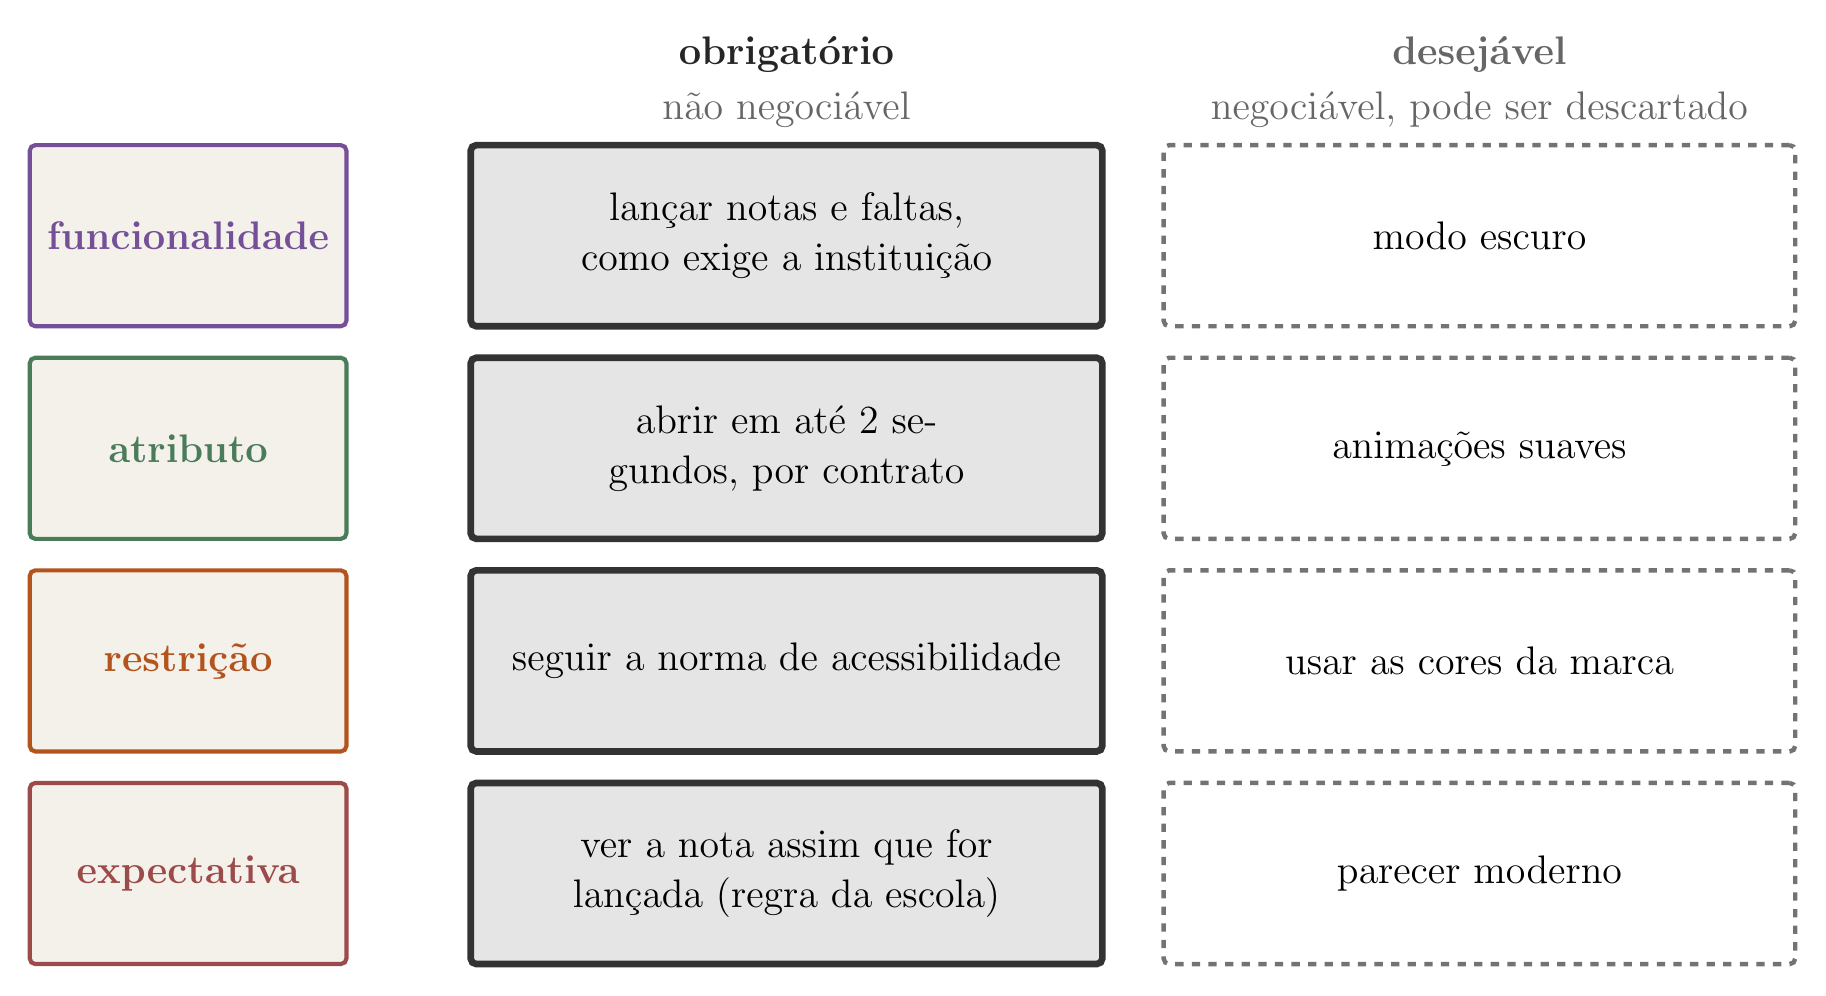
\begin{tikzpicture}[x=1cm,y=1cm]
  \tikzset{rot/.style={dbox, text width=3.6cm, minimum height=2.3cm, font=\Large, line width=1.5pt}}
  \tikzset{ob/.style={dbox, draw=black!80, fill=black!10, line width=2.4pt, text width=7.6cm, minimum height=2.3cm, font=\Large}}
  \tikzset{de/.style={dbox, draw=black!55, fill=white, dashed, line width=1.6pt, text width=7.6cm, minimum height=2.3cm, font=\Large}}
  \node[font=\Large\bfseries, black!85] at (8.6,12.1) {obrigatório};
  \node[font=\Large, black!60] at (8.6,11.4) {não negociável};
  \node[font=\Large\bfseries, black!60] at (17.4,12.1) {desejável};
  \node[font=\Large, black!60] at (17.4,11.4) {negociável, pode ser descartado};
  \node[rot, draw=dblue] at (1.0,9.8) {\textbf{\textcolor{dblue}{funcionalidade}}};
  \node[rot, draw=dgreen] at (1.0,7.1) {\textbf{\textcolor{dgreen}{atributo}}};
  \node[rot, draw=dorange] at (1.0,4.4) {\textbf{\textcolor{dorange}{restrição}}};
  \node[rot, draw=dred] at (1.0,1.7) {\textbf{\textcolor{dred}{expectativa}}};
  \node[ob] at (8.6,9.8) {lançar notas e faltas, como exige a instituição};
  \node[de] at (17.4,9.8) {modo escuro};
  \node[ob] at (8.6,7.1) {abrir em até 2 segundos, por contrato};
  \node[de] at (17.4,7.1) {animações suaves};
  \node[ob] at (8.6,4.4) {seguir a norma de acessibilidade};
  \node[de] at (17.4,4.4) {usar as cores da marca};
  \node[ob] at (8.6,1.7) {ver a nota assim que for lançada (regra da escola)};
  \node[de] at (17.4,1.7) {parecer moderno};
\end{tikzpicture}
\end{document}
